% ------------------------------------------------------------------------------
% TYPO3 CMS 7.4 - What's New - Chapter "Introduction" (English Version)
%
% @author	Michael Schams <schams.net>
% @license	Creative Commons BY-NC-SA 3.0
% @link		http://typo3.org/download/release-notes/whats-new/
% @language	English
% ------------------------------------------------------------------------------
% LTXE-CHAPTER-UID:		9dc37b9a-9fad14c3-bf7eabfd-82b83622
% LTXE-CHAPTER-NAME:	Introduction
% ------------------------------------------------------------------------------

\section{Introduzione}
\begin{frame}[fragile]
	\frametitle{Introduzione}

	\begin{center}\huge{Introduzione}\end{center}
	\begin{center}\huge{\color{typo3darkgrey}\textbf{I fatti in breve}}\end{center}

\end{frame}

% ------------------------------------------------------------------------------
% LTXE-SLIDE-START
% LTXE-SLIDE-UID:		52dbbe60-3d26a833-2754e714-4120d7fa
% LTXE-SLIDE-ORIGIN:	3cc566cf-d7166203-45a36415-7c8e8ebf English
% LTXE-SLIDE-ORIGIN:	5d8622ac-37911548-171bf8ec-5add4ed5 German
% LTXE-SLIDE-TITLE:		TYPO3 CMS 7.4 - The Facts
% ------------------------------------------------------------------------------
\begin{frame}[fragile]
	\frametitle{Introduzione}
	\framesubtitle{TYPO3 CMS 7.4 - I fatti in breve}

	\begin{itemize}
		\item Data di rilascio: 4 agosto 2015
		\item Tipo di rilascio: "Sprint Release"
		\item Visione: Embrace, Innovate, Deliver
		\item Focus principale: Revisione Backend Vol. 2
	\end{itemize}

\end{frame}

% ------------------------------------------------------------------------------
% LTXE-SLIDE-START
% LTXE-SLIDE-UID:		7917290a-6b985c80-fdc387c1-24c6bb12
% LTXE-SLIDE-ORIGIN:	6746e3bc-a8575d0c-e1681766-d0d78911 English
% LTXE-SLIDE-ORIGIN:	9da27f39-55d99c31-9ee9136a-20d96c0e German
% LTXE-SLIDE-TITLE:		System Requirements
% ------------------------------------------------------------------------------
\begin{frame}[fragile]
	\frametitle{Introduzione}
	\framesubtitle{Requisiti di sistema}

	\begin{itemize}
		\item PHP*:\tabto{2.2cm}v5.5.0 - v5.6.x
		\item MySQL:\tabto{2.2cm}v5.5.x - v5.6.x (no strict mode)
		\item Spazio disco:\tabto{2.2cm}min 200 MB
		\item Impostazioni PHP:

			\begin{itemize}
				\item memory\_limit >= 128M
				\item max\_execution\_time >= 240s
				\item l'opzione di compilazione \texttt{--disable-ipv6} \underline{non} deve essere usata
			\end{itemize}

		\item Il Backend richiede IE >= 9 o qualsiasi altro browser moderno

	\end{itemize}

	\vspace{1cm}
	*) Altri dettagli: \href{http://typo3.org/news/article/php-minimum-requirements-for-typo3-cms-7/}{Requisiti minimi PHP per TYPO3 CMS 7}

\end{frame}

% ------------------------------------------------------------------------------
% LTXE-SLIDE-START
% LTXE-SLIDE-UID:		13cf21ed-e19efe9b-6a485ddb-29af556d
% LTXE-SLIDE-ORIGIN:	081f8b1d-b8f58841-dccf8d1d-148fd25d English
% LTXE-SLIDE-ORIGIN:	dbbfebbe-fb43ddb8-bca9ae69-716b8a0f German
% LTXE-SLIDE-TITLE:		Development And Release Timeline
% ------------------------------------------------------------------------------
\begin{frame}[fragile]
	\frametitle{Introduzione}
	\framesubtitle{Sviluppo e tempi di rilascio}

	\begin{figure}
		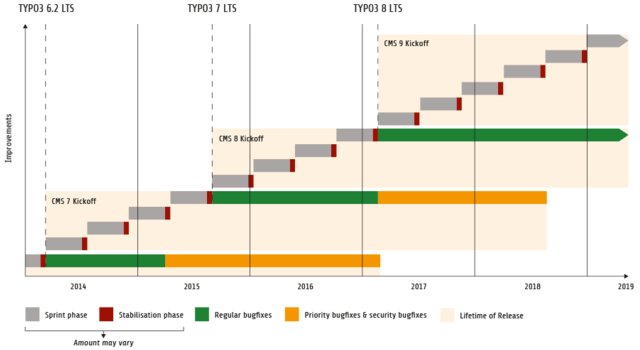
\includegraphics[width=0.90\linewidth]{Introduction/ReleaseAgenda.png}
	\end{figure}

\end{frame}

% ------------------------------------------------------------------------------
% LTXE-SLIDE-START
% LTXE-SLIDE-UID:		d4f32d2e-ba64289a-0f759b2b-4e6b3492
% LTXE-SLIDE-ORIGIN:	a5555bb0-f1f8031f-f271766a-2dbc1b08 English
% LTXE-SLIDE-ORIGIN:	e359142e-e7c10774-5d851da9-b26a275b German
% LTXE-SLIDE-TITLE:		TYPO3 CMS Roadmap
% ------------------------------------------------------------------------------
\begin{frame}[fragile]
	\frametitle{Introduzione}
	\framesubtitle{TYPO3 CMS Roadmap}

	Date di rilascio stimate e loro obiettivo principale:

	\begin{itemize}
		\item v7.0 \tabto{1.0cm}02/Dec/2014\tabto{3.4cm}Revisione Backend Vol. 1
		\item v7.1 \tabto{1.0cm}24/Feb/2015\tabto{3.4cm}Pulizia core \& ottimizzazioni
		\item v7.2 \tabto{1.0cm}28/Apr/2015\tabto{3.4cm}Frontend
		\item v7.3 \tabto{1.0cm}16/Giu/2015\tabto{3.4cm}Ecosistema Pacchetti, Composer\newline
			\tabto{3.4cm}e gestione estensioni
		\item
			\begingroup
				\color{typo3orange}
					v7.4 \tabto{1.0cm}04/Ago/2015\tabto{3.4cm}Revisione Backend Vol. 2
			\endgroup

		\item v7.5 \tabto{1.0cm}29/Sep/2015\tabto{3.4cm}\textit{(da determinare...)}
		\item v7.6 \tabto{1.0cm}xx/xxx/2015\tabto{3.4cm}\textbf{TYPO3 CMS 7 LTS} (Long Term Release)
	\end{itemize}

	\smaller
		\url{https://typo3.org/typo3-cms/roadmap/}\newline
		\url{http://typo3.org/news/article/embrace-and-innovate-typo3-cms-7/}
	\normalsize

\end{frame}

% ------------------------------------------------------------------------------
% LTXE-SLIDE-START
% LTXE-SLIDE-UID:		b64b868c-0f1ca7d9-fe0c6f07-eb82627b
% LTXE-SLIDE-ORIGIN:	5ef3ad6d-b72464d3-6a2867a6-298cb382 English
% LTXE-SLIDE-ORIGIN:	c8966352-3e5159b9-f0e3ea35-9d4455ef German
% LTXE-SLIDE-TITLE:		Installation
% ------------------------------------------------------------------------------
\begin{frame}[fragile]
	\frametitle{Introduzione}
	\framesubtitle{Installazione}

	\begin{itemize}
		\item Procedura ufficiale di installazione su Linux/Mac OS X\newline
			(DocumentRoot ad esempio \texttt{/var/www/site/htdocs}):
		\begin{lstlisting}
			$ cd /var/www/site
			$ wget --content-disposition get.typo3.org/7.4
			$ tar xzf typo3_src-7.4.0.tar.gz
			$ cd htdocs
			$ ln -s ../typo3_src-7.4.0 typo3_src
			$ ln -s typo3_src/index.php
			$ ln -s typo3_src/typo3
			$ touch FIRST_INSTALL
		\end{lstlisting}

		\item Link simbolici in Microsoft Windows:

			\begin{itemize}
				\item Use \texttt{junction} in Windows XP/2000
				\item Use \texttt{mlink} in Windows Vista and Windows 7
			\end{itemize}

	\end{itemize}
\end{frame}

% ------------------------------------------------------------------------------
% LTXE-SLIDE-START
% LTXE-SLIDE-UID:		431db366-29c5811f-e8e6b2fb-b691b180
% LTXE-SLIDE-ORIGIN:	12551741-9cb07199-fb3614d0-1a242a5f English
% LTXE-SLIDE-ORIGIN:	af099855-2b970b2b-89ed7d02-7219b2b9 German
% LTXE-SLIDE-TITLE:		Upgrade to TYPO3 CMS 7
% ------------------------------------------------------------------------------
\begin{frame}[fragile]
	\frametitle{Introduzione}
	\framesubtitle{Aggiornamento a TYPO3 CMS 7.x}

	\begin{itemize}
		\item Aggiornamenti possibili solo da TYPO3 CMS 6.2 LTS
		\item TYPO3 CMS < 6.2 deve essere prima aggiornato a TYPO3 CMS 6.2 LTS
	\end{itemize}

	\begin{itemize}

		\item Istruzioni per l'aggiornamento:\newline
			\smaller\url{http://wiki.typo3.org/Upgrade#Upgrading_to_7.4}\normalsize
		\item Guida ufficiale TYPO3 "TYPO3 Installation and Upgrading":
			\smaller\url{http://docs.typo3.org/typo3cms/InstallationGuide}\normalsize
		\item Approcio generale:
			\begin{itemize}
				\item Verifica i requisiti minimi di sistema \small(PHP, MySQL, etc.)
				\item Verifica \textbf{deprecation\_*.log} nella vecchia istanza TYPO3
				\item Aggiorna tutte le estensioni all'ultima versione
				\item Imposta il nuovo sorgente ed esegui Install Tool \textrightarrow Upgrade Wizard
				\item Verifica modulo startup per gli utente di backend (opzionale)
			\end{itemize}
	\end{itemize}

\end{frame}

% ------------------------------------------------------------------------------
